%-------------------------------------------------------------------------------
%	PACKAGES AND OTHER DOCUMENT CONFIGURATIONS
%-------------------------------------------------------------------------------

\documentclass[11pt]{article}

% Packages
% Packages

% \usepackage{fancyhdr} % Required for custom headers
% \usepackage{lastpage} % Required to determine the last page for the footer
% \usepackage{extramarks} % Required for headers and footers
% \usepackage[usenames,dvipsnames]{color} % Required for custom colors
\usepackage{graphicx} % Required to insert images
% \usepackage{listings} % Required for insertion of code
% \usepackage{courier} % Required for the courier font
% \usepackage{dsfont} % For special math characters
% \usepackage{verbatim}

%\usepackage{amsmath, amssymb, bm} % For matrix notation
\usepackage[english]{babel}
\usepackage[paperwidth=8.5in,paperheight=11in,margin=1.0in]{geometry}
\usepackage{listings}
\usepackage{hyperref}
%\usepackage[cmex10]{amsmath, bm}
\usepackage{amsmath, bm}
\usepackage{blkarray}








% formatting
\pdfcompresslevel0

% ==============================================================================
% PYTHON
% ==============================================================================
\usepackage[utf8]{inputenc}

% Default fixed font does not support bold face
\DeclareFixedFont{\ttb}{T1}{txtt}{bx}{n}{12} % for bold
\DeclareFixedFont{\ttm}{T1}{txtt}{m}{n}{12}  % for normal

% Custom colors
\usepackage{color}
\definecolor{deepblue}{rgb}{0,0,0.5}
\definecolor{deepred}{rgb}{0.6,0,0}
\definecolor{deepgreen}{rgb}{0,0.5,0}

\usepackage{listings}

% Python style for highlighting
\newcommand\pythonstyle{\lstset{
language=Python,
basicstyle=\ttm,
otherkeywords={self},             % Add keywords here
keywordstyle=\ttb\color{deepblue},
emph={MyClass,__init__},          % Custom highlighting
emphstyle=\ttb\color{deepred},    % Custom highlighting style
stringstyle=\color{deepgreen},
frame=tb,                         % Any extra options here
showstringspaces=false,            % 
breaklines=true
}}


% Python environment
\lstnewenvironment{python}[1][]
{\pythonstyle\lstset{#1}
}
{}

% Python for external files
\newcommand\pythonexternal[2][]{{
\pythonstyle\lstinputlisting[#1]{#2}}}

% Python for inline
\newcommand\pythoninline[1]{{\pythonstyle\lstinline!#1!}}
% ==============================================================================
% ==============================================================================

% Margins
\topmargin=-0.45in
\evensidemargin=0in
\oddsidemargin=0in
\textwidth=6.5in
\textheight=9.0in
\headsep=0.25in

\linespread{1.1} % Line spacing

% Set up the header and footer
\pagestyle{fancy}
\lhead{\hmwkAuthorName} % Top left header
\chead{\hmwkClass\ (\hmwkClassInstructor\ \hmwkClassTime): \hmwkTitle} % Top center head
\rhead{\firstxmark} % Top right header
\lfoot{\lastxmark} % Bottom left footer
\cfoot{} % Bottom center footer
\rfoot{Page\ \thepage\ of\ \protect\pageref{LastPage}} % Bottom right footer
\renewcommand\headrulewidth{0.4pt} % Size of the header rule
\renewcommand\footrulewidth{0.4pt} % Size of the footer rule

\setlength\parindent{0pt} % Removes all indentation from paragraphs

%----------------------------------------------------------------------------------------
%	DOCUMENT STRUCTURE COMMANDS
%	Skip this unless you know what you're doing
%----------------------------------------------------------------------------------------

% Header and footer for when a page split occurs within a problem environment
\newcommand{\enterProblemHeader}[1]{\nobreak\extramarks{#1}{#1 continued on next page\ldots}\nobreak\nobreak\extramarks{#1 (continued)}{#1 continued on next page\ldots}\nobreak}

% Header and footer for when a page split occurs between problem environments
\newcommand{\exitProblemHeader}[1]{\nobreak\extramarks{#1 (continued)}{#1 continued on next page\ldots}\nobreak\nobreak\extramarks{#1}{}\nobreak}

\setcounter{secnumdepth}{0} % Removes default section numbers
\newcounter{homeworkProblemCounter} % Creates a counter to keep track of the number of problems

\newcommand{\homeworkProblemName}{}
\newenvironment{homeworkProblem}[1][Problem \arabic{homeworkProblemCounter}]{ % Makes a new environment called homeworkProblem which takes 1 argument (custom name) but the default is "Problem #"
\stepcounter{homeworkProblemCounter} % Increase counter for number of problems
\renewcommand{\homeworkProblemName}{#1} % Assign \homeworkProblemName the name of the problem
\section{\homeworkProblemName} % Make a section in the document with the custom problem count
\enterProblemHeader{\homeworkProblemName} % Header and footer within the environment
}{\exitProblemHeader{\homeworkProblemName} % Header and footer after the environment
}

% Defines the problem answer command with the content as the only argument
\newcommand{\problemAnswer}[1]{\noindent\framebox[\columnwidth, resolution=600][c]{\begin{minipage}{0.98\columnwidth, resolution=600}#1\end{minipage}}}
% Makes the box around the problem answer and puts the content inside }

\newcommand{\homeworkSectionName}{}
\newenvironment{homeworkSection}[1]{ % New environment for sections within homework problems, takes 1 argument - the name of the section
\renewcommand{\homeworkSectionName}{#1} % Assign \homeworkSectionName to the name of the section from the environment argument
\subsection{\homeworkSectionName} % Make a subsection with the custom name of the subsection
\enterProblemHeader{\homeworkProblemName\ [\homeworkSectionName]} % Header and footer within the environment
}{
\enterProblemHeader{\homeworkProblemName} % Header and footer after the environment
}



%-------------------------------------------------------------------------------
%	NAME AND CLASS SECTION
%-------------------------------------------------------------------------------

\newcommand{\hmwkTitle}{HW 8} % Assignment title
\newcommand{\hmwkDueDate}{Thursday, Oct. 16} % Due date
\newcommand{\hmwkClass}{Stat 860} % Course/class
\newcommand{\hmwkClassTime}{4:00 PM} % Class/lecture time
\newcommand{\hmwkClassInstructor}{Grace Wahba} % Teacher/lecturer
\newcommand{\hmwkAuthorName}{Elijah Bernstein-Cooper} % Your name

%-------------------------------------------------------------------------------
%	TITLE PAGE
%-------------------------------------------------------------------------------

\title{\vspace{0in}
    \textmd{\textbf{\hmwkClass:\ \hmwkTitle}}\\
    \normalsize\vspace{0.1in}\small{Due\ on\ \hmwkDueDate}\\
    \vspace{0.1in}\large{\textit{\hmwkClassInstructor\ \hmwkClassTime}}
    \vspace{0.2in}}

\author{\textbf{Elijah Bernstein-Cooper}}
\date{\today} % Insert date here if you want it to appear below your name

%-------------------------------------------------------------------------------

\begin{document}

\maketitle
%\newpage

%===============================================================================
%-------------------------------------------------------------------------------
%	PROBLEM 1
%-------------------------------------------------------------------------------
\begin{homeworkProblem}

    \begin{homeworkSection}{1a}
        See Figure 1 for a plot of $f(x)$ and the smoothing spline. $f(x)$
        consists of three Gaussians superimposed on one another across $x =
        1$ to $x = 100$, with varying means, heights, and widths. We then
        added normal random error to $f(x)$ to be equal to 1\% the maximum
        of $f(x)$. We found that the residual, $R(\lambda) = 2 \times
        10^{-5}$, and the inefficiency, $I = R(\lambda)/R(\lambda_*) =
        2.16$. The optimal $\lambda_*$ was determined empirically, simply by
        testing a range of $\lambda$ values to smooth the spline fit, until the
        residual was minimized.\\

        \begin{figure}[!ht]
           
            \begin{centering}
                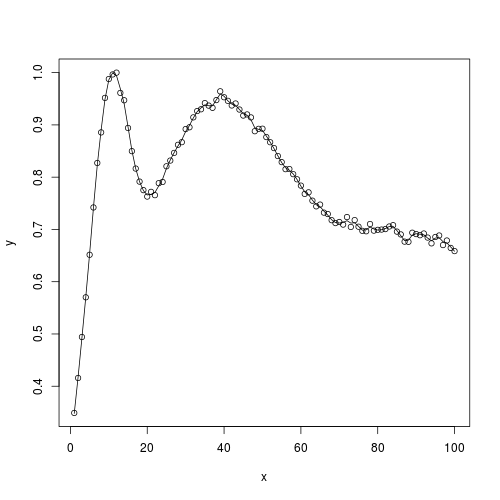
\includegraphics[scale=0.8]{hw8_1a_f_vs_x.png}

                \caption{Plot of noisy function $f(x)$ and the fitted spline
                using generalized cross validation, $f_{\hat{\lambda}}(x)$.}

            \end{centering}
        \end{figure}

        \pythonexternal{hw8_1a.r}

    \end{homeworkSection}

    \begin{homeworkSection}{1b}

        We ran a monte carlo simulation of fitting splines to $f(x)$ 20 times
        for different sets of random noise of the same standard deviation in
        the same way as in problem 1b. We performed this simulation with two
        standard deviations of noise, one at 10\% and one at 1\% the peak of
        $f(x)$. Additionally we performed the experiment for varying number of
        samples of $f(x)$, for $n$ = 32, 64, 128, 256, and 512. For each
        simulation run, we derived the residual $R(\lambda)$, the optimal
        residual $R(\lambda_*)$, and the inefficiency $I$. Figure 2 shows the
        distribution of residuals for different simulations. Figure 3 shows the
        mean residual of a simulation as a function of the sampling number $n$.
        We can see from Figure 3 that for a smaller noise, the spline fit
        more quickly converges than for a larger noise, seeing as the change in
        residual values is small as a function of $n$ in the case of the lower
        noise.

        \begin{figure}[!ht]
            \begin{centering}
                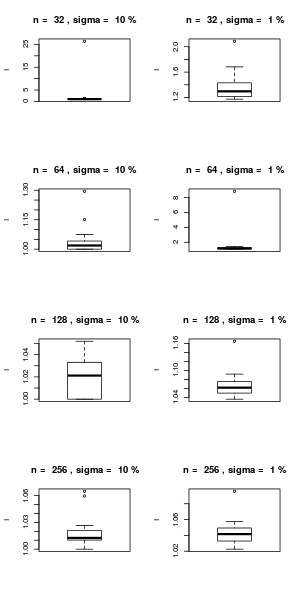
\includegraphics[scale=1]{hw8_1b_Rdist.png}

                \caption{Box plot representations of the distributions of the
                residuals for various sampling numbers, $n$, and noise
            strengths, $\sigma$}

            \end{centering}
        \end{figure}

        \begin{figure}[!ht]
            
            \begin{centering}
                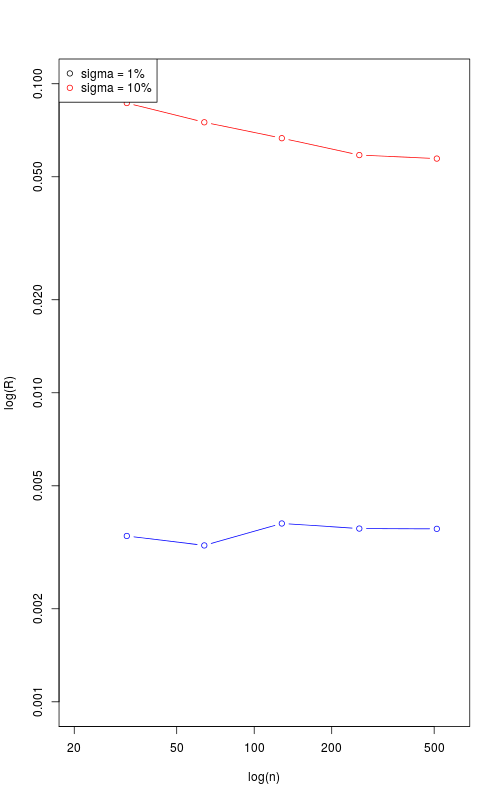
\includegraphics[scale=0.6]{hw8_1b_logR_vs_logn.png}

                \caption{The mean residual of a simulation as a function of the
                    sampling number $n$.  We can see that for a smaller noise,
                    the spline fit more quickly converges than for a larger
                    noise, seeing as the change in residual values is small as
                a function of $n$ in the case of the lower noise. The residuals
            do show a power-like slope as a function of the sampling size,
        where log$R \sim$ constant $-p$\,log$n$.}

            \end{centering}
        \end{figure}

        \pythonexternal{hw8_2.r}

    \end{homeworkSection}

\end{homeworkProblem}
%===============================================================================

\clearpage

%===============================================================================
%-------------------------------------------------------------------------------
%	PROBLEM 2
%-------------------------------------------------------------------------------
\begin{homeworkProblem}
    
    We performed similar monte carlo simulations as in problem 1b for the same
    sampling numbers, and only for one value of the added noise standard
    deviation equal to 50\% of the peak function value. Figure 4 shows the
    distribution of residuals for the different simulations. Figure 5 shows the
    mean residual of a simulation as a function of the sampling number $n$. We
    can see from comparing Figure 3 with Figure 5 that the larger noise
    provides a much steeper slope in $R(n)$

        \begin{figure}[!ht]
            \begin{centering}
                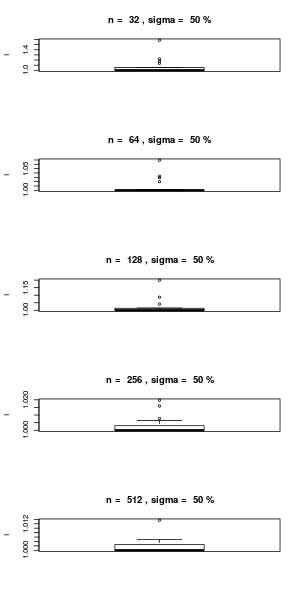
\includegraphics[scale=1]{hw8_2_Rdist.png}

                \caption{Box plot representations of the distributions of the
                    residuals for various sampling numbers, $n$, $\sigma =
                    50\%$max($f$).}

            \end{centering}
        \end{figure}

        \begin{figure}[!ht]
            
            \begin{centering}
                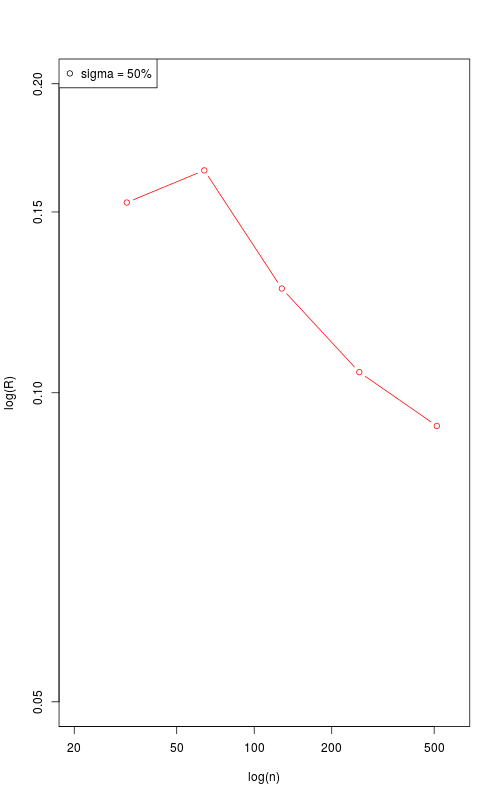
\includegraphics[scale=0.6]{hw8_2_logR_vs_logn.png}

                \caption{The mean residual of a simulation as a function of the
                    sampling number $n$. We can see that for a smaller noise,
                    the spline fit more quickly converges than for a larger
                    noise, seeing as the change in residual values is small as
                a function of $n$ in the case of the lower noise, as compared
            with Figure 3. The residuals do show a power-like slope as a
        function of the sampling size, where log$R \sim$ constant $-p$\,log$n$.}

            \end{centering}
        \end{figure}

        \pythonexternal{hw8_2.r}

\end{homeworkProblem}
%===============================================================================

\end{document}

